% chapter03.tex - 张量与张量代数
\chapter{张量与张量代数 (Tensors and Tensor Algebra)}
\label{chap:tensor}

\section{从物理直觉到切向量}

\begin{note}[物理动机]
在经典力学中，粒子的速度是一个向量——它有大小和方向。在弯曲时空中，我们仍然需要描述"速度"、"动量"、"力"等物理量。但问题在于：在弯曲流形上，我们无法像在 $\mathbb{R}^n$ 中那样直接将两点"相减"来得到一个向量——因为流形上不同的点并不自然地属于同一个向量空间（我们可以"放大"某点，但每个点有自己独立的切空间）。因此，我们需要一个\textbf{局部的}、与坐标选择无关的向量定义。这就是切向量的概念 \cite{Carroll1997,Reall_Part3_GR}。
\end{note}

\subsection{切向量的三种等价定义}

光滑流形 $M$ 在点 $p$ 处的\textbf{切向量} (tangent vector) 是流形在该点的"无穷小位移"的数学抽象。我们可以用三种等价的方式来定义它：

\begin{definition}[切向量：导子定义]
设 $p \in M$。点 $p$ 处的一个\textbf{切向量}是一个线性映射 $v: C^\infty(M) \to \mathbb{R}$，满足 Leibniz 法则：
\begin{equation}
    v(fg) = v(f) \cdot g(p) + f(p) \cdot v(g), \quad \forall f,g \in C^\infty(M).
\end{equation}
切向量本质上是一个"\textbf{在点 $p$ 处的方向导数算符}"。它接受一个光滑函数，返回该函数沿切向量方向的变化率。
\end{definition}

\begin{definition}[切向量：曲线定义]
设 $\gamma: (-\varepsilon, \varepsilon) \to M$ 是一条通过 $p = \gamma(0)$ 的光滑曲线。曲线 $\gamma$ 在 $p$ 处的\textbf{切向量}是作用在函数上的导数算符：
\begin{equation}
    v_\gamma(f) = \left.\frac{\dd}{\dd t} (f \circ \gamma)(t)\right|_{t=0}.
\end{equation}
两条曲线定义了同一个切向量，当且仅当它们在任意坐标卡下的一阶 Taylor 展开一致。
\end{definition}

\begin{definition}[切向量：坐标定义]
在坐标卡 $(U, \phi = (x^1,\ldots,x^n))$ 中，$n$ 个偏导数算符 $\{\pd_1|_p, \ldots, \pd_n|_p\}$（其中 $\pd_\mu|_p f = \frac{\pd}{\pd x^\mu}(f \circ \phi^{-1})(\phi(p))$）构成 $T_pM$ 的一组基。任意切向量可唯一地表示为：
\begin{equation}
    v = v^\mu \, \pd_\mu|_p,
\end{equation}
其中 $v^\mu \in \mathbb{R}$ 称为 $v$ 在坐标卡 $\phi$ 下的\textbf{分量}。
\end{definition}

这三种定义是等价的：导子定义最抽象但最几何化；曲线定义最直观（"切向量就是曲线的速度"）；坐标定义最便于计算。物理学家通常在具体的坐标系中计算，但始终记得分量 $v^\mu$ 和基 $\pd_\mu$ 的组合才能给出与坐标无关的几何量。

\begin{figure}[htbp]
\centering
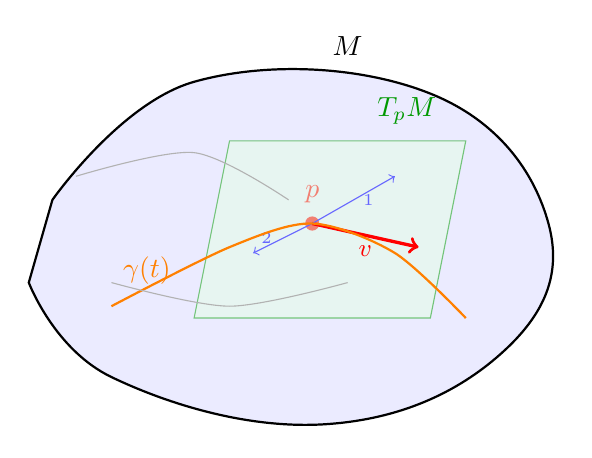
\begin{tikzpicture}[scale=1.5]
    % Manifold M (curved surface)
    \draw[thick,fill=blue!8] plot[smooth,tension=0.7] coordinates {
        (-2.0,0.5) (-0.8,1.5) (1.2,1.4) (2.2,0.3) 
        (1.8,-0.8) (0.3,-1.4) (-1.5,-1.0) (-2.2,-0.2)
    } -- cycle;
    \node at (0.5,1.8) {$M$};
    
    % Point p
    \fill[red] (0.2,0.3) circle (0.06);
    \node[red] at (0.2,0.55) {$p$};
    
    % Tangent plane at p
    \draw[green!60!black,fill=green!10,opacity=0.5] 
        (-0.8,-0.5) -- (1.2,-0.5) -- (1.5,1.0) -- (-0.5,1.0) -- cycle;
    \node[green!60!black] at (1.0,1.25) {$T_pM$};
    
    % Tangent vector
    \draw[->,red,very thick] (0.2,0.3) -- (1.1,0.1) 
        node[midway,below,font=\small] {$v$};
    
    % Coordinate basis
    \draw[->,blue!60] (0.2,0.3) -- (0.9,0.7) 
        node[midway,right,font=\small] {$\pd_1$};
    \draw[->,blue!60] (0.2,0.3) -- (-0.3,0.05) 
        node[midway,left,font=\small] {$\pd_2$};
    
    % Curve through p
    \draw[orange,thick] plot[smooth] coordinates {
        (-1.5,-0.4) (-0.5,0.1) (0.2,0.3) (0.9,0.05) (1.5,-0.5)
    };
    \node[orange] at (-1.2,-0.1) {$\gamma(t)$};
    
    % Flow lines on manifold
    \draw[gray!60,thin] plot[smooth] coordinates {
        (-1.8,0.7) (-0.8,0.9) (0.0,0.5)
    };
    \draw[gray!60,thin] plot[smooth] coordinates {
        (-1.5,-0.2) (-0.5,-0.4) (0.5,-0.2)
    };
\end{tikzpicture}
\caption{二维流形 $M$ 在点 $p$ 处的切空间 $T_pM$。$T_pM$ 是流形在 $p$ 点的"最佳线性近似"——一个二维向量平面。切向量 $v$ 可以分解为坐标基 $\{\pd_1,\pd_2\}$ 的线性组合。通过 $p$ 的曲线 $\gamma(t)$ 在 $p$ 点的切向量正是 $v$。}
\label{fig:tangent_space}
\end{figure}

\subsection{切空间与坐标变换}

\begin{definition}[切空间]
点 $p \in M$ 处所有切向量的集合记作 $T_pM$，称为 $M$ 在 $p$ 点的\textbf{切空间} (tangent space)。$T_pM$ 是一个 $n$ 维实向量空间，其维数与流形 $M$ 的维数相同。
\end{definition}

\begin{property}[切向量的坐标变换]
设 $(U, x^\mu)$ 和 $(\tilde{U}, \tilde{x}^\mu)$ 是包含 $p$ 的两个坐标卡。同一向量 $v \in T_pM$ 在两组坐标系的分量之间的变换规则为：
\begin{equation}
    \tilde{v}^\mu = \frac{\pd \tilde{x}^\mu}{\pd x^\nu} \, v^\nu, \quad v^\mu = \frac{\pd x^\mu}{\pd \tilde{x}^\nu} \, \tilde{v}^\nu.
\end{equation}
其中 Jacobi 矩阵 $\frac{\pd \tilde{x}^\mu}{\pd x^\nu}$ 在点 $p$ 处取值。这就是物理学中著名的\textbf{逆变变换律} (contravariant transformation law)——"逆变"意味着分量变换的方式与基向量的变换方式"相反"。
\end{property}

\begin{remark}[为什么称为"逆变"？]
坐标基向量 $\pd_\mu$ 在坐标变换下按 $\pd_\mu = \frac{\pd \tilde{x}^\nu}{\pd x^\mu} \tilde{\pd}_\nu$ 变换（系数是 Jacobi 矩阵的转置），而切向量的分量 $v^\mu$ 按 $\tilde{v}^\mu = \frac{\pd \tilde{x}^\mu}{\pd x^\nu} v^\nu$ 变换（系数是 Jacobi 矩阵本身）。这两种变换"方向相反"——因此被称为"逆"变（contra-variant）。与之相对，余向量的分量按协变 (co-variant) 方式变换：$\tilde{\omega}_\mu = \frac{\pd x^\nu}{\pd \tilde{x}^\mu} \omega_\nu$。
\end{remark}

\subsection{余切空间与余向量}

\begin{definition}[余切空间]
切空间 $T_pM$ 的\textbf{对偶空间} (dual space) 记作 $T_p^*M$，称为 $M$ 在 $p$ 点的\textbf{余切空间} (cotangent space)。$T_p^*M$ 中的元素 $\omega$ 是切空间上的线性泛函：
\begin{equation}
    \omega: T_pM \to \mathbb{R}, \quad \omega(av + bw) = a \, \omega(v) + b \, \omega(w).
\end{equation}
$T_p^*M$ 中的元素称为\textbf{余向量} (covector) 或 \textbf{1-形式} (1-form) \cite{Reall_Part3_GR}。
\end{definition}

一个特别重要的余向量是函数的\textbf{全微分}。对任意光滑函数 $f \in C^\infty(M)$，其在 $p$ 点的微分 $\dd f|_p \in T_p^*M$ 定义为：
\begin{equation}
    (\dd f|_p)(v) = v(f), \quad \forall v \in T_pM.
\end{equation}
在坐标卡中，$\{\dd x^1|_p, \ldots, \dd x^n|_p\}$ 构成 $T_p^*M$ 的一组基（称为坐标余基），且满足对偶关系：
\begin{equation}
    \dd x^\mu|_p (\pd_\nu|_p) = \delta^\mu_\nu.
\end{equation}

\begin{property}[余向量的坐标变换]
余向量 $\omega \in T_p^*M$ 的分量在坐标变换下的变换规则为：
\begin{equation}
    \tilde{\omega}_\mu = \frac{\pd x^\nu}{\pd \tilde{x}^\mu} \, \omega_\nu.
\end{equation}
这称为\textbf{协变变换律} (covariant transformation law)。注意这里的系数是逆 Jacobi 矩阵 $\frac{\pd x^\nu}{\pd \tilde{x}^\mu}$，而非正 Jacobi 矩阵。
\end{property}

\subsection{切丛与向量场}

\begin{definition}[切丛与向量场]
流形 $M$ 的\textbf{切丛} (tangent bundle) 是所有切空间的不交并：
\begin{equation}
    TM = \bigsqcup_{p \in M} T_pM.
\end{equation}
$TM$ 本身是一个 $2n$ 维光滑流形。$M$ 上的一个\textbf{光滑向量场} $X$ 是切丛的一个光滑截面，即对每个 $p \in M$，光滑地指定一个切向量 $X_p \in T_pM$。$M$ 上全体光滑向量场的集合记作 $\mathfrak{X}(M)$。
\end{definition}

\begin{remark}
切丛的概念在现代物理学中广泛出现：粒子的\textbf{相空间}是位形空间的余切丛 $T^*Q$；规范场是主丛上的联络；Higgs 场是伴丛的截面。所有这些构造都建立在切丛和余切丛的基础之上。
\end{remark}

\section{张量的定义与张量代数}

\subsection{从多重线性映射到张量}

余向量将单个切向量映射为实数。自然的推广是考虑接受多个切向量和余向量的多重线性映射——这就是\textbf{张量}。

\begin{definition}[$(r,s)$ 型张量]
点 $p \in M$ 处的一个 $(r,s)$ 型\textbf{张量} (tensor) 是一个多重线性映射：
\begin{equation}
    T: \underbrace{T_p^*M \times \cdots \times T_p^*M}_{r \text{ 个副本}} \times \underbrace{T_pM \times \cdots \times T_pM}_{s \text{ 个副本}} \to \mathbb{R},
\end{equation}
它在每一个变量上都是线性的。$r$ 称为\textbf{逆变阶数} (contravariant order)，$s$ 称为\textbf{协变阶数} (covariant order)，总阶数 $r+s$ 称为张量的\textbf{秩} (rank)。
\end{definition}

在分量表示中，$(r,s)$ 型张量由 $n^{r+s}$ 个分量 $T^{\mu_1\cdots\mu_r}{}_{\nu_1\cdots\nu_s}$ 完全确定，这些分量满足特定的坐标变换规则（见下文）。

\begin{figure}[htbp]
\centering
\begin{tikzpicture}[scale=1.1]
    % Title
    \node[font=\large\bfseries] at (0,2.5) {张量的可视化};
    
    % (0,0) type - scalar
    \fill[blue!30] (-3,1) circle (0.6);
    \node at (-3,1) {$f$};
    \node at (-3,0.2) {标量 $(0,0)$};
    
    % (1,0) type - vector
    \draw[->,red,very thick] (0,1) -- (1.5,1.8);
    \fill[red] (0,1) circle (0.06);
    \node at (1.0,2.1) {$v^\mu$};
    \node at (0.5,0.2) {向量 $(1,0)$};
    
    % (0,1) type - covector
    \draw[green!50!black,very thick] (3,1.8) -- (4.5,1);
    \draw[green!50!black,dashed] (3,1) -- (3,1.8);
    \draw[green!50!black,dashed] (4.5,1) -- (4.5,1.8);
    \node at (4.0,1.0) {$\omega_\mu$};
    \node at (3.5,0.2) {余向量 $(0,1)$};
    
    % (0,2) type - metric
    \draw[blue!60,thick] (-3,-0.5) -- (-4.5,-1.5);
    \draw[blue!60,thick] (-3,-0.5) -- (-2.5,-1.8);
    \draw[blue!60,thick] (-3,-0.5) -- (-1.2,-1.3);
    \node at (-3,-2.2) {度规 $g_{\mu\nu}$ $(0,2)$};
    
    % (1,1) type - linear map
    \draw[->,purple,thick] (1.5,-0.5) -- (0.5,-1.5);
    \fill[purple] (1.5,-0.5) circle (0.06);
    \node at (1.5,-2.2) {线性映射 $L^\mu{}_\nu$ $(1,1)$};
    
    % (1,3) type - Riemann tensor
    \node at (5,-0.5) {$\cdots$};
    \node at (5,-2.2) {$R^\rho{}_{\sigma\mu\nu}$ $(1,3)$};
\end{tikzpicture}
\caption{不同秩的张量对应不同类型的几何对象。标量（秩 0）是流形上的函数；向量（秩 1）是切空间中的元素；度规张量（秩 2）定义了内积；黎曼曲率张量（秩 4）描述了空间的弯曲。张量的阶数越高，编码的几何信息越丰富。}
\label{fig:tensor_types}
\end{figure}

\begin{itemize}
    \item $(0,0)$ 型：标量函数 $f \in C^\infty(M)$——一个不依赖于坐标系选择的数
    \item $(1,0)$ 型：切向量 $v \in T_pM$——流形上的"方向"
    \item $(0,1)$ 型：余向量 $\omega \in T_p^*M$——切向量上的线性泛函
    \item $(1,1)$ 型：线性变换 $L: T_pM \to T_pM$——如能量-动量张量的"1上1下"形式
    \item $(0,2)$ 型：双线性型——度规张量 $g_{\mu\nu}$ 是典型例子
    \item $(2,0)$ 型：逆度规 $g^{\mu\nu}$——在缩并中与度规配对
    \item $(1,3)$ 型：黎曼曲率张量 $R^\rho{}_{\sigma\mu\nu}$——编码了所有曲率信息
\end{itemize}

\subsection{张量积}

\begin{definition}[张量积]
设 $T$ 是 $(r,s)$ 型张量，$S$ 是 $(p,q)$ 型张量。其\textbf{张量积} (tensor product) $T \otimes S$ 是一个 $(r+p, s+q)$ 型张量，定义为：
\begin{equation}
    (T \otimes S)^{\mu_1\cdots\mu_r\nu_1\cdots\nu_p}{}_{\rho_1\cdots\rho_s\sigma_1\cdots\sigma_q}
    = T^{\mu_1\cdots\mu_r}{}_{\rho_1\cdots\rho_s} \, S^{\nu_1\cdots\nu_p}{}_{\sigma_1\cdots\sigma_q}.
\end{equation}
\end{definition}

\begin{remark}[张量代数的分次结构]
全体张量构成一个\textbf{分次代数} (graded algebra)：$\mathcal{T}(M) = \bigoplus_{r,s \geq 0} \mathcal{T}^{(r,s)}(M)$。分次乘法的规则是 $\mathcal{T}^{(r,s)} \otimes \mathcal{T}^{(p,q)} \subseteq \mathcal{T}^{(r+p,s+q)}$。张量积满足结合性，但不交换（除非其中一个张量的秩为 0）\cite{TensorFields2017}。这种分次结构使得张量代数成为一个强大的代数系统——物理量在相互作用下"增加阶数"，但系统始终保持在张量代数的框架内。
\end{remark}

\subsection{缩并：指标的求和}

\begin{definition}[缩并]
设 $T$ 是 $(r,s)$ 型张量（$r \geq 1$, $s \geq 1$）。对第 $i$ 个逆变指标和第 $j$ 个协变指标进行\textbf{缩并} (contraction) 得到一个 $(r-1, s-1)$ 型张量。在分量形式下：
\begin{equation}
    (\operatorname{tr}_{ij} T)^{\mu_1\cdots\hat{\mu}_i\cdots\mu_r}{}_{\nu_1\cdots\hat{\nu}_j\cdots\nu_s}
    = T^{\mu_1\cdots\lambda\cdots\mu_r}{}_{\nu_1\cdots\lambda\cdots\nu_s},
\end{equation}
其中 $\hat{\cdot}$ 表示被移除的指标，Einstein 求和约定意味着对重复指标 $\lambda$ 自动求和 \cite{Reall_Part3_GR}。
\end{definition}

\begin{itemize}
    \item 线性变换的迹：$\operatorname{tr}(L) = L^\mu{}_\mu$（$(1,1)$ 型缩并为 $(0,0)$ 型标量）
    \item 向量与余向量的自然配对：$\omega(v) = \omega_\mu v^\mu$（$(0,1)$ 与 $(1,0)$ 缩并）
    \item 里奇张量：$R_{\mu\nu} = R^\lambda{}_{\mu\lambda\nu}$（$(1,3)$ 型的一次缩并为 $(0,2)$ 型）
    \item 标量曲率：$R = g^{\mu\nu} R_{\mu\nu}$（先缩并再缩并 = 两次缩并）
\end{itemize}

\begin{remark}
缩并的本质是"求和"——将一个逆变指标和一个协变指标配对后求和，从而消去这两个指标。从几何上看，缩并对应的是"取迹"操作。缩并是唯一能够自然地（即与基的选择无关地）将不同指标"配对"的方式。值得注意的是，你不能将两个逆变指标（或两个协变指标）直接缩并——你需要先用度规升降其中一个指标。
\end{remark}

\subsection{抽象指标记法}

现代微分几何和广义相对论中广泛使用\textbf{抽象指标记法} (abstract index notation)，由 Penrose 推广 \cite{Reall_Part3_GR}。在这一记法中，张量 $T$ 写为 $T^{ab}{}_{c}$（其中拉丁字母 $a,b,c$ 是抽象指标），但这些指标并不代表某个特定坐标系下的分量——它们只是"标记张量槽位"的标签。

这种记法的优势在于：它允许我们使用指标运算的简便性，同时保持几何的不变性。方程 $T^{ab}{}_{c} = U^{a}{}_{cd} V^{bd}$ 既是几何陈述（"两个张量相等"），又是分量计算指令（"对指标进行缩并求和"）。在广义相对论和量子场论中，希腊字母 $\mu,\nu$ 通常表示具体坐标下的分量，拉丁字母 $a,b,c$ 表示抽象指标。

\section{张量的坐标变换规则}

张量的定义特性是其分量在坐标变换下的变换规则。这是张量概念的"操作定义"。

\begin{property}[张量变换律]
设 $T$ 是 $(r,s)$ 型张量。在坐标变换 $x \mapsto \tilde{x}$ 下，其分量变换为：
\begin{equation}
    \tilde{T}^{\mu_1\cdots\mu_r}{}_{\nu_1\cdots\nu_s}
    = \frac{\pd \tilde{x}^{\mu_1}}{\pd x^{\rho_1}} \cdots \frac{\pd \tilde{x}^{\mu_r}}{\pd x^{\rho_r}}
    \cdot \frac{\pd x^{\sigma_1}}{\pd \tilde{x}^{\nu_1}} \cdots \frac{\pd x^{\sigma_s}}{\pd \tilde{x}^{\nu_s}}
    \cdot T^{\rho_1\cdots\rho_r}{}_{\sigma_1\cdots\sigma_s}.
\end{equation}
\end{property}

这条规则告诉我们：每一个上指标乘以 Jacobi 矩阵 $\frac{\pd \tilde{x}}{\pd x}$，每一个下指标乘以逆 Jacobi 矩阵 $\frac{\pd x}{\pd \tilde{x}}$。

\begin{remark}[如何判断一个量是不是张量]
在广义相对论中，一个最基本的直观判别法是：如果一个多重指标的量在坐标变换下按照上述规则变换，它就是一个张量；否则就不是。这是张量的\textbf{操作定义}。特别地，Christoffel 符号 $\Gamma^\lambda{}_{\mu\nu}$ 不按张量的方式变换（它多出了一项二阶导数的非齐次项），因此它\textbf{不是}张量——这个事实在后续章节中将反复强调。
\end{remark}

\section{对称张量与反对称张量}

\begin{definition}[对称与反对称张量]
一个 $(0,2)$ 型张量 $T_{\mu\nu}$ 称为：
\begin{itemize}
    \item \textbf{对称的} (symmetric)，如果 $T_{\mu\nu} = T_{\nu\mu}$
    \item \textbf{反对称的} (antisymmetric/skew-symmetric)，如果 $T_{\mu\nu} = -T_{\nu\mu}$
\end{itemize}
\end{definition}

对称化与反对称化操作可以推广到任意 $(0,k)$ 型张量：

\begin{definition}[对称化与反对称化]
对 $(0,k)$ 型张量 $T_{\mu_1\cdots\mu_k}$：
\begin{align}
    T_{(\mu_1\cdots\mu_k)} &= \frac{1}{k!} \sum_{\sigma \in S_k} T_{\mu_{\sigma(1)}\cdots\mu_{\sigma(k)}}, \quad\text{（对称化：$k!$ 个排列的平均）} \
    T_{[\mu_1\cdots\mu_k]} &= \frac{1}{k!} \sum_{\sigma \in S_k} \operatorname{sgn}(\sigma) \, T_{\mu_{\sigma(1)}\cdots\mu_{\sigma(k)}}, \quad\text{（反对称化：$k!$ 个带符号排列的平均）}
\end{align}
其中 $S_k$ 是 $k$ 个元素的置换群，$\operatorname{sgn}(\sigma)$ 是置换的符号（偶置换为 $+1$，奇置换为 $-1$）。
\end{definition}

\begin{property}[反对称张量的独立分量数]
$n$ 维空间上的 $(0,k)$ 型完全反对称张量的独立分量数为 $\binom{n}{k} = \frac{n!}{k!(n-k)!}$。特别地，$k > n$ 时反对称张量恒为零（因为没有足够的维度来产生非零的完全反对称组合）。
\end{property}

\section{度规张量：连接几何与物理}

度规张量是微分几何与广义相对论中最重要的张量——它将流形的微分拓扑结构转化为有"长度"和"角度"的黎曼几何结构。

\begin{definition}[度规张量]
$M$ 上的一个\textbf{度规张量} (metric tensor) $g$ 是一个对称的、非退化的 $(0,2)$ 型光滑张量场：
\begin{equation}
    g = g_{\mu\nu} \, \dd x^\mu \otimes \dd x^\nu, \quad g_{\mu\nu} = g_{\nu\mu}, \quad \det(g_{\mu\nu}) \neq 0.
\end{equation}
\end{definition}

度规张量赋予流形上每一点切空间中的一个内积（可能是不定的）：
\begin{equation}
    \langle u, v \rangle_g = g_{\mu\nu} u^\mu v^\nu.
\end{equation}

\begin{definition}[号差与洛伦兹流形]
在标准正交基下，度规的对角元素中正负号的数量差称为度规的\textbf{号差} (signature)。如果号差为 $(-,+,+,+)$ 或 $(+,-,-,-)$，则称度规具有\textbf{洛伦兹号差} (Lorentzian signature)。配备了洛伦兹度规的流形称为\textbf{洛伦兹流形}。在广义相对论中，时空被建模为一个四维洛伦兹流形 $(\mathcal{M}, g)$ \cite{Wald1984}。
\end{definition}

根据号差，切向量可以分类为：
\begin{itemize}
    \item $g_{\mu\nu} v^\mu v^\nu < 0$：\textbf{类时} (timelike) —— 物理粒子的世界线
    \item $g_{\mu\nu} v^\mu v^\nu = 0$：\textbf{类光} (lightlike/null) —— 光子的世界线
    \item $g_{\mu\nu} v^\mu v^\nu > 0$：\textbf{类空} (spacelike) —— 不能因果相连的事件间隔
\end{itemize}

\begin{definition}[逆度规]
由非退化性，度规矩阵 $g_{\mu\nu}$ 可逆。其逆记作 $g^{\mu\nu}$，满足 $g^{\mu\lambda} g_{\lambda\nu} = \delta^\mu_\nu$。$g^{\mu\nu}$ 是一个 $(2,0)$ 型对称张量，称为\textbf{逆度规} (inverse metric)。
\end{definition}

度规和逆度规提供了指标升降的标准方式：
\begin{equation}
    v_\mu = g_{\mu\nu} v^\nu, \quad T^{\mu\nu} = g^{\mu\rho} g^{\nu\sigma} T_{\rho\sigma}, \quad R = g^{\mu\nu} R_{\mu\nu}.
\end{equation}
指标升降使得我们可以在协变形式和逆变形式之间自由切换，这是张量分析中最常用的技术操作。

\begin{note}[物理意义]
在广义相对论中，度规张量扮演着双重角色：
\begin{enumerate}
    \item \textbf{几何角色}：它定义了时空中"距离"的概念——类时曲线上的固有时间隔 $\dd \tau^2 = -g_{\mu\nu} \dd x^\mu \dd x^\nu / c^2$
    \item \textbf{动力学角色}：度规是引力场的\textbf{动力学变量}——爱因斯坦场方程是关于 $g_{\mu\nu}$ 的偏微分方程。在这个意义上，度规就是"引力势"的广义相对论推广。
\end{enumerate}
\end{note}

\begin{itemize}
    \item \textbf{闵可夫斯基度规}（平坦时空）：
    \begin{equation}
        \dd s^2 = -\dd t^2 + \dd x^2 + \dd y^2 + \dd z^2, \quad g_{\mu\nu} = \operatorname{diag}(-1, +1, +1, +1)
    \end{equation}
    \item \textbf{施瓦西度规}（球对称黑洞外部）：
    \begin{equation}
        \dd s^2 = -\left(1 - \frac{2GM}{r}\right) \dd t^2 + \left(1 - \frac{2GM}{r}\right)^{-1} \dd r^2 + r^2(\dd\theta^2 + \sin^2\theta\,\dd\phi^2)
    \end{equation}
    注意：当 $M=0$ 时，施瓦西度规在 $r \to \infty$ 处约化为闵可夫斯基度规——这体现了广义相对论在弱场极限下回到狭义相对论。
\end{itemize}

\section{张量密度}

许多重要的物理量（如拉格朗日密度 $\sqrt{-g} \Lag$、作用量中的体积元 $\sqrt{-g} \dd^4 x$）涉及度规的行列式。这引入了张量密度的概念。

\begin{definition}[张量密度]
一个\textbf{权重为 $w$ 的 $(r,s)$ 型张量密度}（或称为相对张量）是一个在坐标变换下按照以下规则变换的多重指标量：
\begin{equation}
    \tilde{\mathfrak{T}}^{\mu_1\cdots}{}_{\nu_1\cdots}
    = \left|\det\!\left(\frac{\pd x}{\pd \tilde{x}}\right)\right|^{w}
    \frac{\pd \tilde{x}^{\mu_1}}{\pd x^{\rho_1}} \cdots
    \mathfrak{T}^{\rho_1\cdots}{}_{\sigma_1\cdots}.
\end{equation}
特别地，$\sqrt{-g}$ 是权重为 $+1$ 的标量密度；$1/\sqrt{-g}$ 是权重为 $-1$ 的标量密度。
\end{definition}

\begin{remark}
在广义相对论中，体积元 $\dd^4 x$ 本身不是标量（在坐标变换下它乘上 Jacobi 行列式），但组合 $\sqrt{-g} \, \dd^4 x$ 是一个真正的标量。这使得作用量 $S = \int \Lag \sqrt{-g} \, \dd^4 x$ 在任意坐标变换下都是不变的——物理定律的协变性由此得到保证。
\end{remark}

\section{Levi-Civita 张量与定向}

\begin{definition}[Levi-Civita 符号与张量]
\textbf{Levi-Civita 符号} $\tilde{\varepsilon}_{\mu_1\cdots\mu_n}$ 是满足 $\tilde{\varepsilon}_{12\cdots n} = +1$ 且关于任意两个指标的交换完全反对称的量。然而它\textbf{不是}一个张量——它是一个权重为 $-1$ 的张量密度。

真正的\textbf{Levi-Civita 张量}（或体积元形式）是：
\begin{equation}
    \varepsilon_{\mu_1\cdots\mu_n} = \sqrt{|g|} \, \tilde{\varepsilon}_{\mu_1\cdots\mu_n}, \quad
    \varepsilon^{\mu_1\cdots\mu_n} = \frac{1}{\sqrt{|g|}} \, \tilde{\varepsilon}^{\mu_1\cdots\mu_n}.
\end{equation}
其中 $g = \det(g_{\mu\nu})$。注意 $\varepsilon_{\mu_1\cdots\mu_n}$ 是真正的 $(0,n)$ 型反对称张量。
\end{definition}

Levi-Civita 张量在广义相对论的多处都出现：体积分（$\dd V = \varepsilon_{\mu_1\cdots\mu_n} \dd x^{\mu_1} \wedge \cdots \wedge \dd x^{\mu_n}$）、Hodge 对偶（第 \ref{chap:forms} 章）、以及在引力作用量中引入 Gauss--Bonnet 拓扑项。

\section{算例演练 (Worked Examples)}

下面通过大量具体算例来巩固本章的所有核心概念。所有算例均尽可能详细地展示中间步骤。

\subsection{Einstein 求和约定}

\
\begin{equation}
    A^\mu B_\mu = A^0 B_0 + A^1 B_1 + A^2 B_2 + A^3 B_3.
\end{equation}
重复的上下指标 $\mu$ 自动求和，求和范围由时空维数决定（此处四维）。注意 $A^\mu$ 和 $A_\mu$ 是不同的对象（逆变 vs 协变）。

\
\begin{equation}
    \delta^\mu_\mu = \delta^0_0 + \delta^1_1 + \delta^2_2 + \delta^3_3 = 1 + 1 + 1 + 1 = 4.
\end{equation}
Kronecker delta 的完全缩并等于时空维数 $n$。在 $n$ 维空间中：$\delta^\mu_\mu = n$。这在迹运算中经常用到。

\
\begin{equation}
    \delta^\mu_\nu A^\nu = A^\mu.
\end{equation}
这是因为 $\delta^\mu_\nu = 1$ 仅当 $\mu = \nu$，因此求和只剩下 $\nu = \mu$ 的一项。$\delta^\mu_\nu$ 的作用是"替换指标"。

\
设 Minkowski 度规 $\eta_{\mu\nu} = \text{diag}(-1,+1,+1,+1)$，计算 $\eta_{\mu\nu} \eta^{\mu\nu}$：
\begin{equation}
    \eta_{\mu\nu} \eta^{\mu\nu} = \eta_{\mu\nu} \eta^{\mu\nu} = \delta^\mu_\mu = 4.
\end{equation}
更详细地：
\begin{equation}
    \eta^{\mu\nu} \eta_{\nu\rho} = \delta^\mu_\rho.
\end{equation}
验证 $\mu = 0, \rho = 0$：$\eta^{0\nu} \eta_{\nu 0} = \eta^{00} \eta_{00} = (-1) \times (-1) = 1 = \delta^0_0$。$\checkmark$

\
\begin{equation}
    g_{\mu\nu} A^\mu B^\nu = A_0 B_0 - A_1 B_1 - A_2 B_2 - A_3 B_3 \quad \text{（号差 $(-,+,+,+)$）}.
\end{equation}
展开：$g_{00}A^0 B^0 + g_{11}A^1 B^1 + g_{22}A^2 B^2 + g_{33}A^3 B^3 = -A^0 B^0 + A^1 B^1 + A^2 B^2 + A^3 B^3$。

\begin{remark}[求和约定的哑指标与自由指标]
在表达式中，重复且配对（一上一下或两个都在位置不变的情况下由度规连接）的指标称为\textbf{哑指标} (dummy index)，可以任意重命名而不改变含义。例如 $A_\mu B^\mu = A_\nu B^\nu$。未配对的指标（如 $A^\mu$ 中的 $\mu$）称为\textbf{自由指标} (free index)，等式两侧必须匹配。
\end{remark}

\subsection{张量积算例}

\
设 $A^\mu = (1, 2, 0, -1)$ 和 $B^\mu = (0, 3, 1, 0)$ 为 Minkowski 时空中的两个切向量。其张量积 $T^{\mu\nu} = A^\mu B^\nu$ 是一个 $(2,0)$ 型张量，分量为 $4 \times 4 = 16$ 个：
\begin{equation}
    T^{\mu\nu} = A^\mu B^\nu = 
    \begin{pmatrix}
        0 & 3  & 1  & 0 \\
        0 & 6  & 2  & 0 \\
        0 & 0  & 0  & 0 \\
        0 & -3 & -1 & 0
    \end{pmatrix}.
\end{equation}
其中 $T^{01} = A^0 B^1 = 1 \times 3 = 3$，$T^{10} = A^1 B^0 = 2 \times 0 = 0$，等等。注意 $T^{\mu\nu} \neq T^{\nu\mu}$ 一般情况（张量积不交换）。

\
度规 $g_{\mu\nu}$ 是 $(0,2)$ 型，切向量 $V^\rho$ 是 $(1,0)$ 型。其张量积 $S^\rho{}_{\mu\nu} = V^\rho g_{\mu\nu}$ 是一个 $(1,2)$ 型张量，有 $4 \times 4 \times 4 = 64$ 个分量。具体写出一项：
\begin{equation}
    S^1{}_{00} = V^1 g_{00} = V^1 \times (-1) = -V^1.
\end{equation}

\
将 $\delta^\mu_\nu$（$(1,1)$ 型）与向量 $V^\rho$ 做张量积：
\begin{equation}
    W^{\mu\rho}{}_{\nu} = \delta^\mu_\nu V^\rho.
\end{equation}
然后对 $\mu$ 和 $\nu$ 缩并：$W^{\mu\rho}{}_{\mu} = \delta^\mu_\mu V^\rho = 4 V^\rho$。迹使结果放大了 $n$ 倍。

\subsection{缩并算例}

\
设 $L^\mu{}_\nu$ 是一个 $(1,1)$ 型张量，表示为 $4 \times 4$ 矩阵。其缩并（迹）为：
\begin{equation}
    \text{tr}(L) = L^\mu{}_\mu = L^0{}_0 + L^1{}_1 + L^2{}_2 + L^3{}_3.
\end{equation}
具体数值例子：若 $L^\mu{}_\nu = \text{diag}(2, -1, 3, 0)$，则 $\text{tr}(L) = 2 + (-1) + 3 + 0 = 4$。

\
里奇张量 $R_{\mu\nu}$ 是 Riemann 张量的缩并 $R^\lambda{}_{\mu\lambda\nu}$。在四维中：
\begin{equation}
    R_{00} = R^0{}_{000} + R^1{}_{010} + R^2{}_{020} + R^3{}_{030}.
\end{equation}
每一项都是 Riemann 张量的一个具体分量。例如 $R^1{}_{010}$ 表示沿 $x^0$ 和 $x^1$ 方向的曲率对 $x^1$ 基向量的效应。

\
从里奇张量进一步缩并得到标量曲率 $R = g^{\mu\nu} R_{\mu\nu}$：
\begin{equation}
    \begin{aligned}
        R &= g^{00} R_{00} + g^{11} R_{11} + g^{22} R_{22} + g^{33} R_{33} \
          &= -R_{00} + R_{11} + R_{22} + R_{33} \quad \text{（Minkowski 背景）}.
    \end{aligned}
\end{equation}

\subsection{坐标变换算例}

\
设 $\mathbb{R}^2$ 上，笛卡尔坐标 $(x, y)$ 与极坐标 $(r, \theta)$ 的关系为 $x = r\cos\theta$, $y = r\sin\theta$。一个切向量 $V$ 在笛卡尔坐标系下的分量为 $V^x, V^y$，在极坐标下的分量 $V^r, V^\theta$ 由逆变变换律给出：
\begin{equation}
    \begin{pmatrix} V^r \\[2pt] V^\theta \end{pmatrix}
    = \begin{pmatrix}
        \frac{\pd r}{\pd x} & \frac{\pd r}{\pd y} \\[6pt]
        \frac{\pd \theta}{\pd x} & \frac{\pd \theta}{\pd y}
    \end{pmatrix}
    \begin{pmatrix} V^x \\[2pt] V^y \end{pmatrix}.
\end{equation}
计算 Jacobi 矩阵：由 $r = \sqrt{x^2 + y^2}$ 得 $\frac{\pd r}{\pd x} = \frac{x}{r} = \cos\theta$, $\frac{\pd r}{\pd y} = \frac{y}{r} = \sin\theta$。由 $\theta = \arctan(y/x)$ 得 $\frac{\pd \theta}{\pd x} = -\frac{y}{r^2} = -\frac{\sin\theta}{r}$, $\frac{\pd \theta}{\pd y} = \frac{x}{r^2} = \frac{\cos\theta}{r}$。因此：
\begin{equation}
    \boxed{V^r = \cos\theta \, V^x + \sin\theta \, V^y, \quad V^\theta = -\frac{\sin\theta}{r} V^x + \frac{\cos\theta}{r} V^y}.
\end{equation}
这正是向量在极坐标下的分量——注意 $\theta$ 分量的量纲是 $\text{radian}/\text{长度}$，因为基向量 $\pd_\theta$ 本身带有长度量纲。

\
一个标量函数 $f(x,y) = x^2 + y^2 = r^2$ 的梯度 $\dd f$ 是余向量。在笛卡尔坐标下：$\omega_x = \pd_x f = 2x$, $\omega_y = \pd_y f = 2y$。在极坐标下由协变变换律：
\begin{equation}
    \begin{aligned}
        \omega_r &= \frac{\pd x}{\pd r} \omega_x + \frac{\pd y}{\pd r} \omega_y = \cos\theta \cdot 2x + \sin\theta \cdot 2y = 2r, \
        \omega_\theta &= \frac{\pd x}{\pd \theta} \omega_x + \frac{\pd y}{\pd \theta} \omega_y = (-r\sin\theta) \cdot 2x + (r\cos\theta) \cdot 2y = 0.
    \end{aligned}
\end{equation}
验证：$\dd f = 2r \dd r$——极坐标下梯度的 $\theta$ 分量为零，因为 $f$ 是径向对称的。

\
设 $F_{\mu\nu}$ 是 $(0,2)$ 型反对称张量，在坐标系 $x^\mu = (t, x, y, z)$ 下非零分量为 $F_{01} = E_x$, $F_{02} = E_y$, $F_{12} = -B_z$。在沿 $x$ 方向的 Lorentz boost 下，
\begin{equation}
    \tilde{t} = \gamma(t - vx), \quad \tilde{x} = \gamma(x - vt), \quad \tilde{y} = y, \quad \tilde{z} = z,
\end{equation}
其中 $\gamma = 1/\sqrt{1-v^2}$。计算 $\tilde{F}_{01}$：
\begin{equation}
    \tilde{F}_{01} = \frac{\pd x^\rho}{\pd \tilde{t}} \frac{\pd x^\sigma}{\pd \tilde{x}} F_{\rho\sigma}.
\end{equation}
非零贡献来自 Jacobi 矩阵元素。最终得到 $\tilde{F}_{01} = E_x$（不变量），$\tilde{F}_{02} = \gamma(E_y - v B_z)$——这正是电磁场在 Lorentz 变换下的变换公式（电场的一部分转化为磁场）。\textbf{张量的变换律自动给出了物理量的坐标变换}。

\subsection{对称化与反对称化算例}

\
任何 $(0,2)$ 型张量 $T_{\mu\nu}$ 可唯一分解为：
\begin{equation}
    T_{\mu\nu} = T_{(\mu\nu)} + T_{[\mu\nu]}, \quad T_{(\mu\nu)} = \frac{1}{2}(T_{\mu\nu} + T_{\nu\mu}), \quad T_{[\mu\nu]} = \frac{1}{2}(T_{\mu\nu} - T_{\nu\mu}).
\end{equation}
例如 $T_{\mu\nu} = \begin{pmatrix} 0 & 2 & -1 \ 1 & 0 & 3 \ 0 & -2 & 0 \end{pmatrix}$（以矩阵表示）。则：
\begin{equation}
    T_{(\mu\nu)} = \begin{pmatrix} 0 & 1.5 & -0.5 \ 1.5 & 0 & 0.5 \ -0.5 & 0.5 & 0 \end{pmatrix}, \quad
    T_{[\mu\nu]} = \begin{pmatrix} 0 & 0.5 & -0.5 \ -0.5 & 0 & 2.5 \ 0.5 & -2.5 & 0 \end{pmatrix}.
\end{equation}
验证：$T_{(\mu\nu)} + T_{[\mu\nu]} = T_{\mu\nu}$。$\checkmark$

\
在 $n=3$ 维空间中，$(0,3)$ 型完全反对称张量的独立分量数为 $\binom{3}{3} = 1$——只有一个独立分量！具体设 $A_{[\mu\nu\rho]}$，则所有非零分量都由 $A_{123}$ 决定：
\begin{equation}
    A_{123} = A_{231} = A_{312} = -A_{132} = -A_{213} = -A_{321}.
\end{equation}
因此 $A_{\mu\nu\rho} = A_{123} \cdot \tilde{\varepsilon}_{\mu\nu\rho}$，其中 $\tilde{\varepsilon}$ 是 Levi-Civita 符号。这正是三维空间中\textbf{轴向量} (pseudovector) 对应到 2-形式的数学基础（如磁场 $\mathbf{B}$ 对应到 $B_{ij} = \varepsilon_{ijk} B_k$）。

\
因 $g_{\mu\nu} = g_{\nu\mu}$，有：
\begin{equation}
    g_{\mu\nu} A^\mu B^\nu = g_{(\mu\nu)} A^\mu B^\nu = g_{\mu\nu} A^{(\mu} B^{\nu)}.
\end{equation}
第二个等号成立因为反对称部分与对称度规缩并的结果为 0：$g_{\mu\nu} A^{[\mu} B^{\nu]} = 0$。一般规则：$\text{对称} \times \text{反对称} = 0$（在完全缩并下）。

\subsection{指标升降算例}

\
在 Minkowski 时空 $(\eta_{\mu\nu}) = \text{diag}(-1,+1,+1,+1)$ 中，设 $V^\mu = (V^0, V^1, V^2, V^3) = (3, 1, -2, 0)$。降指标：
\begin{equation}
    V_\mu = \eta_{\mu\nu} V^\nu: \quad V_0 = -V^0 = -3, \quad V_1 = V^1 = 1, \quad V_2 = V^2 = -2, \quad V_3 = V^3 = 0.
\end{equation}
即 $V_\mu = (-3, 1, -2, 0)$。再升回去：$V^\mu = \eta^{\mu\nu} V_\nu$ 得到原始分量。$\checkmark$

\
球面度规 $g_{\mu\nu} = \text{diag}(1, \sin^2\theta)$，逆度规 $g^{\mu\nu} = \text{diag}(1, 1/\sin^2\theta)$。设切向量 $V^\mu = (V^\theta, V^\phi) = (2, 3)$。降指标：
\begin{equation}
    V_\theta = g_{\theta\theta} V^\theta = 1 \times 2 = 2, \quad V_\phi = g_{\phi\phi} V^\phi = \sin^2\theta \times 3 = 3\sin^2\theta.
\end{equation}
注意 $V_\phi$ 依赖于 $\theta$——在靠近极点（$\theta \to 0$）时它趋于零。这反映了球面在极点处的坐标奇异性。

\
缩并 $\omega_\mu V^\mu$ 可以先升 $\omega$ 或先降 $V$：
\begin{equation}
    \omega_\mu V^\mu = \omega^\mu V_\mu = g^{\mu\nu} \omega_\mu V_\nu = g_{\mu\nu} \omega^\mu V^\nu.
\end{equation}
数值验证：设 $\omega_\mu = (1, 2, -1, 0)$, $V^\mu = (3, 0, 1, -2)$ 在 Minkowski 时空。$\omega_\mu V^\mu = -1 \times 3 + 2 \times 0 + (-1) \times 1 + 0 \times (-2) = -4$。先升 $\omega$：$\omega^\mu = (-1, 2, -1, 0)$，则 $\omega^\mu V_\mu = (-1) \times (-3) + 2 \times 0 + (-1) \times 1 + 0 \times (-2) = -4$。$\checkmark$

\subsection{度规及逆度规的算例}

\
施瓦西度规（$c=1$, $G=1$）：
\begin{equation}
    g_{\mu\nu} = \text{diag}\!\left(-\left(1-\frac{2M}{r}\right),\; \left(1-\frac{2M}{r}\right)^{-1},\; r^2,\; r^2\sin^2\theta\right).
\end{equation}
逆度规为各对角元的倒数：
\begin{equation}
    g^{\mu\nu} = \text{diag}\!\left(-\left(1-\frac{2M}{r}\right)^{-1},\; 1-\frac{2M}{r},\; \frac{1}{r^2},\; \frac{1}{r^2\sin^2\theta}\right).
\end{equation}
验证缩并：例如 $g^{11} g_{11} = (1-\frac{2M}{r}) \times (1-\frac{2M}{r})^{-1} = 1$。

\
第一章提到的球面 Christoffel 符号 $\Gamma^\phi{}_{\theta\phi} = \cot\theta$ 可以通过 Levi-Civita 公式直接验证：
\begin{equation}
    \Gamma^\phi{}_{\theta\phi} = \frac{1}{2} g^{\phi\rho} (\pd_\theta g_{\phi\rho} + \pd_\phi g_{\theta\rho} - \pd_\rho g_{\theta\phi}).
\end{equation}
由于 $g_{\theta\phi} = 0$，只有 $\rho = \phi$ 项非零：
\begin{equation}
    \Gamma^\phi{}_{\theta\phi} = \frac{1}{2} g^{\phi\phi} \pd_\theta g_{\phi\phi} = \frac{1}{2} \cdot \frac{1}{\sin^2\theta} \cdot 2\sin\theta\cos\theta = \cot\theta. \quad \checkmark
\end{equation}


\begin{note}[物理意义：本章总结]
本章建立的所有张量运算——求和约定、张量积、缩并、坐标变换、对称化/反对称化、指标升降——构成了广义相对论日常计算的语言。在后续章节中：
\begin{itemize}
    \item \textbf{联络系数} $\Gamma^\lambda{}_{\mu\nu}$ 由度规的导数通过升降指标构造（第 \ref{chap:connection} 章）
    \item \textbf{曲率张量} $R^\rho{}_{\sigma\mu\nu}$ 的缩并产生里奇张量和爱因斯坦张量（第 \ref{chap:curvature} 章）
    \item \textbf{测地线方程}使用 Christoffel 符号进行指标缩并（第 \ref{chap:geodesic} 章）
    \item \textbf{爱因斯坦场方程} $G_{\mu\nu} = 8\pi G T_{\mu\nu}$ 中的每一项都是通过张量运算构造的（第 10 章）
\end{itemize}
\end{note}

\begin{figure}[htbp]
\centering
\begin{tikzpicture}[scale=1.2]
    % Left: 笛卡尔坐标
    \draw[->,thick] (-1.5,0) -- (2.5,0) node[right] {$x$};
    \draw[->,thick] (0,-1.5) -- (0,2.5) node[above] {$y$};
    
    % Vector V
    \draw[->,red,very thick] (0,0) -- (2.0,1.0);
    \node[red] at (2.2,1.2) {$V$};
    \node[red,font=\footnotesize] at (1.5,0.3) {$V^\mu=(V^x,V^y)$};
    
    % Grid
    \draw[gray!30,step=0.5] (-1.5,-1.5) grid (2.5,2.5);
    
    % Right: 极坐标
    \draw[->,thick] (5.5,0) -- (9.5,0) node[right] {$r$};
    \draw[->,thick] (7,1.5) -- (7,2.5);
    
    % Radial lines
    \foreach \a in {0,30,...,330} {
        \draw[gray!30] (7,0) -- ++(\a:2.0);
    }
    % Circles
    \foreach \r in {0.5,1.0,1.5,2.0} {
        \draw[gray!30] (7,0) circle (\r);
    }
    
    % Same vector V in polar coords
    \draw[->,red,very thick] (7,0) -- (9.0,1.0);
    \node[red] at (9.2,1.2) {$V$};
    \node[red,font=\footnotesize] at (8.2,0.3) {$\tilde{V}^\mu=(V^r,V^\theta)$};
    
    % Transformation arrow between
    \draw[->,teal,very thick,dashed] (4.5,0.5) -- (5.0,0.5);
    \node[teal] at (3.5,0.8) {$\tilde{V}^\mu = \frac{\pd \tilde{x}^\mu}{\pd x^\nu} V^\nu$};
    
    \node at (0.5,-2.0) {笛卡尔坐标};
    \node at (7.0,-2.0) {极坐标};
\end{tikzpicture}
\caption{同一向量 $V$ 在不同坐标系下的分量表示。左：笛卡尔坐标基 $\{\pd_x,\pd_y\}$ 下的分量 $(V^x, V^y)$。右：极坐标基 $\{\pd_r,\pd_\theta\}$ 下的分量 $(V^r, V^\theta)$。两组分量通过逆变变换律联系：$\tilde{V}^\mu = \frac{\pd \tilde{x}^\mu}{\pd x^\nu} V^\nu$。注意 $V^\theta$ 的量纲与 $V^x$ 不同——因为极坐标基向量 $\pd_\theta$ 的长度随 $r$ 变化。}
\label{fig:tensor_transform}
\end{figure}

\begin{note}[物理意义]
张量是物理学定律的通用语言，而爱因斯坦的广义协变性原理在数学上等价于"所有物理定律必须表达为张量方程"。张量方程的一个关键性质是\textbf{协变性}：如果一个张量方程在一个坐标系中成立，那么它在所有坐标系中都成立——只要你在每个坐标系中正确地计算了分量。这确保了物理定律不依赖于我们选择的描述方式。
\end{note}
